\documentclass[a4paper]{article}
\usepackage[french]{babel}
\usepackage[utf8]{inputenc}
\usepackage[T1]{fontenc}
\usepackage{todonotes}
\usepackage{graphicx}
\usepackage{subcaption}
\usepackage{amssymb} % nécessaire pour \mathbb
\usepackage{mathtools}
\usepackage{csquotes}
\usepackage{hyperref}
\usepackage[style=ieee]{biblatex}
\addbibresource{ref.bib}
\bibliography{ref.bib}

\renewcommand\UrlFont{\color{blue}\rmfamily}

\title{Etat de l'art des réseaux de convolutions de graphes et leurs nuances.}
\author{Cléa HAN - Léa TRIQUET - Adrien ZABBAN}
\date{27 octobre 2023}

\begin{document}
\maketitle

\section{Introduction}

Ce rapport se penche sur trois des méthodes les plus prometteuses et influentes dans le domaine du deep learning avec des graphes :
Graph Convolusional Networks~\cite{DBLP:journals/corr/KipfW16} (GCN), Simplifying Graph Convolutional 
Networks~\cite{DBLP:journals/corr/abs-1902-07153}
(SGC) et les  Graph Isomorphism Network~\cite{DBLP:journals/corr/abs-1810-00826} (GIN). Ces approches ont démontré leur capacité 
à extraire des informations pertinentes à partir de données de graphes, permettant ainsi de résoudre une multitude de problèmes, 
tels que la classification de nœuds, la prédiction de liens, la recommandation de contenu, et bien d'autres.

Au cours de ce rapport, nous explorerons en détail le fonctionnement de ces trois méthodes, en mettant l'accent sur leurs principes 
fondamentaux, leurs avantages et leurs domaines d'application. Nous discuterons également des défis et des opportunités inhérents à 
l'utilisation du deep learning dans des contextes de données de graphes, ainsi que des tendances futures dans ce domaine en constante
évolution.

\section{Les différentes méthodes}

\subsection{Graph Convolusional Networks (GCN)}\label{sec: GCN}
Un Graph Convolution Network (GCN) est un type de réseau de neurones artificiels conçu pour traiter des données 
structurées sous forme de graphes. Ils utilisent des opérations de convolution spécialement adaptées aux graphes 
pour propager l'information entre les nœuds du graphe, ce qui leur permet de capturer les relations et les 
dépendances entre les entités interconnectées. L'équation~\ref{eq: propragation de couche} représente la règle de
propagation de la couche $l$ à la couche $l+1$.
\begin{equation}
    H^{(l-1)} = \sigma (\Tilde{D}^{-\frac{1}{2}} \Tilde{A} \Tilde{D}^{-\frac{1}{2}} H^{(l)} W^{(l)})
    \label{eq: propragation de couche}
\end{equation}
où $\Tilde{A}=A+I_n$ est la matrice d'adjacence au quelle on ajoute des connections sur les noeuds vers 
eux-mêmes. $\Tilde{D_{ii}}=\sum_j{\Tilde{A_{ij}}}$ qui est une matrice diagonale des degrés des noeuds du 
graphe. $W^{(l)}$ sont les poids de la couche $l$ et $H^{(l)}$ est la sortie de la couche $l-1$, $H^{(0)}=X$. 
$\sigma$ est une fonction d'activation.

Par exemple, un petit réseaux de convolutions de graphes pourait suivre l'équation~\ref{eq: reseaux de 2 GCN}
\begin{equation}
    Z_{GCN} = \text{softmax}(\hat{A}\,\text{ReLU}(\hat{A}XW^{(0)})W^{(1)})
    \label{eq: reseaux de 2 GCN}
\end{equation}
où $\hat{A} = \Tilde{D}^{-\frac{1}{2}} \Tilde{A} \Tilde{D}^{-\frac{1}{2}}$


\subsection{Simplifying Graph Convolutional Networks (SGC)}

Les modèles SGCs sont construits à partir d'une linéarisation des GCNs en faisant l'hypothèse que les non linéarités 
principalement apportées par les ReLU entre les différentes couches d'un GCN n'apportent pas d'informations significatives.
Ainsi, les modèles SGCs retirent ces non linéarités et conservent uniquement un Softmax en dernière couche, afin de pouvoir 
obtenir des résultats sous forme d'une distribution de probabilités.

Nous pouvons modéliser le SGC sous la forme de l'expression simplifiée suivante l'équiation~\ref{eq: SGC}
\begin{equation}
  Z_{SGC}=\text{softmax}(\hat{A}^KXW)
  \label{eq: SGC}
\end{equation}
où $\hat{A}^K$ représente les $K$ multiplications successives avec $\hat{A}$ notre matrice d'adjacence normalisée,
définie dans la section~\ref{sec: GCN}, $X$ est les entrées 
et $W$ est la matrice réunissant l'ensemble des poids utilisés dans le modèle tel que : $W=W^{(1)} W^{(2)} \dots W^{(K)}$.
La SGC équivaut à une une composante d'extraction de caractéristiques: $\tilde{X}=\hat{A}^KX$, ce qui nécessite aucun 
poids. Puis, cela est suivi d'une régression logistique $Z_{SGC}=\text{softmax}(\tilde{X}W)$. Ainsi la première étape équivaut 
à du prétraitement des caractéristiques de nos données $X$, car aucun poids n'est appliqué sur nos données. Ainsi, l'entraînement
du SGC s'apparente en réalité à une régression logistique multi classe sur des données prétraités. 
D'autre part, l'entraînement d'une régression logistique est un problème d'optimisation convexe bien documenté, ainsi ses 
performances seront relativement meilleures que celles du GCN qui contient des non linéarités. De plus, l'entraînement du 
SGC sera naturellement plus rapide.
D'un point de vue “graphe”, la SGC correspond à un filtre fixe sur le domaine du graphe spectral. Si nous ajoutons des boucles 
dans le graphe original, l'application du SGC permet de réduire la taille du spectre graphique grâce à l'astuce de renormalisation 
présentée par Kipf \& Welling~\cite{DBLP:journals/corr/KipfW16}. La SGC agit comme un filtre passe bas qui lisse les 
caractéristiques du graphes, ainsi les 
nœuds voisins vont avoir tendance à partager des représentations et donc des prédictions similaires. 


\subsection{Graph Isomorphism Network (GIN)}

Les GIN (Graph Isomorphism Networks) sont une classe de réseaux neuronaux profonds spécialement conçus pour le traitement des données
de graphes. Leur fonctionnement repose sur une idée clé : définir un modèle qui peut apprendre à identifier si deux graphes sont 
isomorphes, c'est-à-dire s'ils ont la même structure sous-jacente. Les GIN commencent par représenter les nœuds et les arêtes d'un
graphe sous forme de vecteurs, puis ils appliquent des couches de réseau neuronal pour agréger et mettre à jour ces représentations.
Les informations de voisinage sont combinées itérativement à chaque couche pour capturer des motifs de plus en plus complexes. 
En fin de compte, le GIN génère un vecteur de représentation pour chaque graphe d'entrée. Cela permet de comparer ces vecteurs 
pour déterminer si les graphes sont isomorphes. L'équation~\ref{eq: GIN} représente la règle de
propagation de la couche $l$ à la couche $l+1$ pour le sommet $v$.

\begin{equation}
    h_v^{(l)} = \text{MLP}^{(l)} \Bigl((1+\epsilon^{(l)}) \cdot h_v^{(l-1)}+\sum_{u\in \mathcal{N}(v)}h_u^{(l-1)}\Bigl)
    \label{eq: GIN}
\end{equation}
où $\text{MLP}$ est un perceptron à plusieurs couches (multi-layer perceptrons), $\epsilon \in~\mathbb{R}$ est un hyperparamètre, 
et $\mathcal{N}(v)$ est l'ensemble des voisins du somment $v$. En notant $A$ la matrice d'adjacence, on peut réécrire 
l'équation~\ref{eq: GIN} sous forme matricielle donnée par la formule~\ref{eq: GINmat}.
\begin{equation}
    h^{(l)} = \text{MLP}^{(l)} \Bigl(( A + (1+\epsilon) \cdot I_n)\cdot h^{(l-1)} \Bigl)
    \label{eq: GINmat}
\end{equation}

\section{Entraînement}
Nous avons entraîné 3 réseaux de neurones utilisant chacun une méthode (GCN, SGC et GIN) sur la base de données ENZYMES de 
TUDataset~\cite{Morris+2020}. Cette base de données contient 600 graphes représentant 6 types d'enzymes différentes. En moyenne
les graphes ont 32 sommets et 124 arrêtes et chaque sommet de chaque graphe est représenté par 3 features. Le but des modèles
de graphes et de trouver le bon type d'enzymes à partir d'un graphe. Dans tous les entraînements, nous avons utilisé la Cross
Entropy pour la fonction de coût, et la métrique accuracy pour voir les performances des réseaux.

\paragraph{GCN:}
Nous avons crée un modèle en concaténant 4 modules GCN à la suite. Nous avons mis des fonctions ReLU entre ces couches, et 
ajouté une couche dense à la fin du réseau pour avoir en sortie un vecteur de taille 6 (le nombre d'enzymes différentes). La 
Figure~\ref{fig: GCN} montre les courbes d'apprentissages pendant 40 epochs.

\begin{figure}[ht]
    \centering
    \begin{subfigure}{0.47\textwidth}
      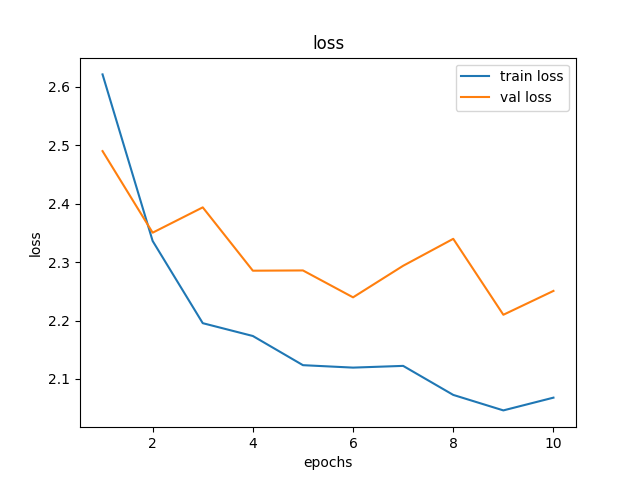
\includegraphics[width=\linewidth]{../results/GCN_0/loss.png}
      \caption{Cross Entropy Loss}
    \end{subfigure}
    \hfill
    \begin{subfigure}{0.47\textwidth}
      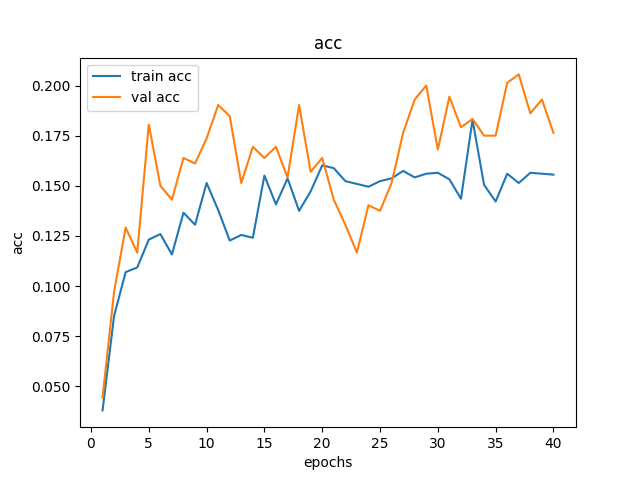
\includegraphics[width=\linewidth]{../results/GCN_0/acc.png}
      \caption{accuracy}
    \end{subfigure}
    \caption{Apprentissage d'un réseau de neurones utilisant les GCN}
    \label{fig: GCN}
\end{figure}

\paragraph{SGC:}
Nous avons concaténé 2 couche de SGC à la suite avec un $K=4$, et mis la fonction ReLU entre. Puis nous avons utilisé une couche
dense à la fin du réseau. La Figure~\ref{fig: SGC} montre les courbes d'apprentissages pendant 40 epochs.

\begin{figure}[ht]
    \begin{subfigure}{0.47\textwidth}
      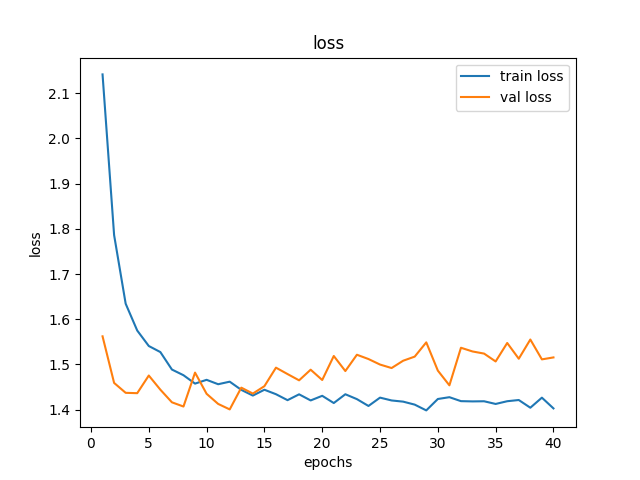
\includegraphics[width=\linewidth]{../results/SGC_1/loss.png}
      \caption{Cross Entropy Loss}
    \end{subfigure}
    \hfill
    \begin{subfigure}{0.47\textwidth}
      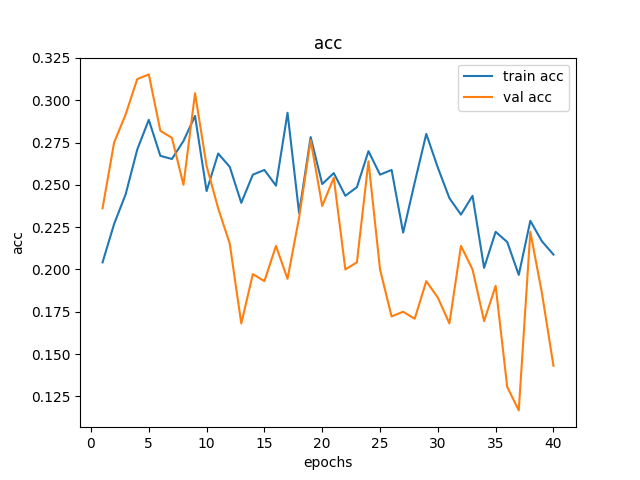
\includegraphics[width=\linewidth]{../results/SGC_1/acc.png}
      \caption{accuracy}
    \end{subfigure}
    \caption{Apprentissage d'un réseau de neurones utilisant les SGC}
    \label{fig: SGC}
\end{figure}

\paragraph{GIN:}
Nous avons concaténé 2 couche de GIN. Sur ces 2 couches, nous avons utilisé un réseau de neurone utilisant 2 couches denses. Nous 
avons mis une activation ReLU entre chaque couche dense. La Figure~\ref{fig: GIN} montre les courbes d'apprentissages pendant
40 epochs. On peut voir que l'apprentissage est assez chaotique, pourtant on a utilisé un faible learning rate (0.001).

\begin{figure}[ht]
    \begin{subfigure}{0.47\textwidth}
      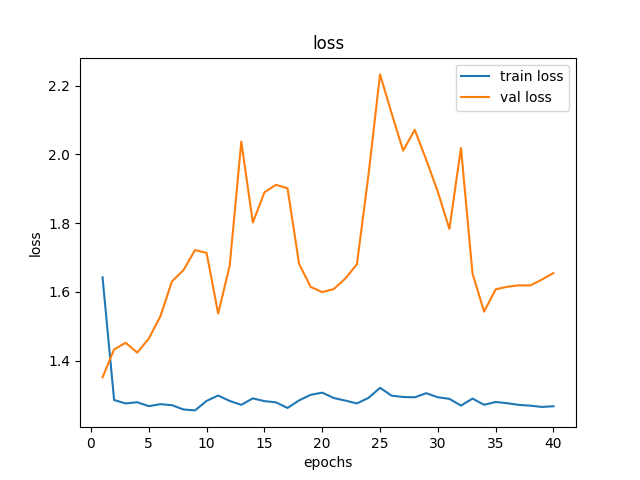
\includegraphics[width=\linewidth]{../results/GIN_3/loss.png}
      \caption{Cross Entropy Loss}
    \end{subfigure}
    \hfill
    \begin{subfigure}{0.47\textwidth}
      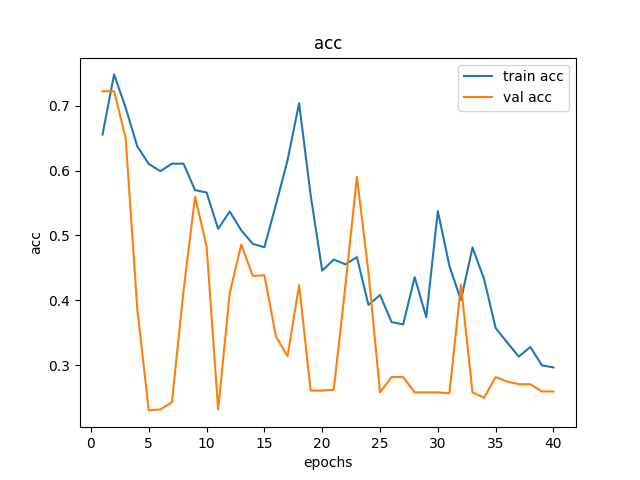
\includegraphics[width=\linewidth]{../results/GIN_3/acc.png}
      \caption{accuracy}
    \end{subfigure}
    \caption{Apprentissage d'un réseau de neurones utilisant les GIN}
    \label{fig: GIN}
\end{figure}

\section{Résultats}

Nous voyons sur la Table~\ref{tab:test}, les résultats des modèles sur la base de données de teste. 

\begin{table}[ht]
    \centering
    \begin{tabular}{|c|c|c|c|}
        \hline
        Modèles & GCN & SGC & GIN \\
        \hline
        Cross Entropy & 2.86 & 1.85 & 1.75 \\
        \hline
        Accuracy & 0.20 & 0.16 & 0.66\\
        \hline
    \end{tabular}
    \caption{Résultat sur la base de données de teste}
    \label{tab:test}
\end{table}

Les données indiquent que le modèle GIN affiche la performance la plus remarquable, avec la plus faible Cross Entropy (1.75) et la 
meilleure Accuracy (0.66). Ce modèle excelle dans la réduction de l'erreur de prédiction et la réalisation de prédictions précises.
En comparaison, SGC et GCN présentent des performances inférieures en termes d'erreur et de précision, avec des valeurs plus élevées
dans les deux métriques. Cependant, il convient de noter que le choix du modèle dépendra du contexte spécifique de la tâche, des 
objectifs et des contraintes de ressources. Dans l'ensemble, ces résultats suggèrent que GIN peut être la meilleure option lorsque 
la précision des prédictions est essentielle, mais d'autres facteurs, tels que la complexité de l'entraînement, doivent également
être pris en compte pour faire un choix éclairé entre les modèles.

\section{Conclusion}
En résumé, ce rapport a exploré en détail trois des méthodes les plus influentes dans le domaine en pleine expansion du deep learning 
avec des graphes : les Graph Convolutional Networks (GCN), les Simplifying Graph Convolutional Networks (SGC), et les Graph Isomorphism
Networks (GIN). Ces méthodes ont été examinées à travers diverses perspectives, notamment leurs principes de fonctionnement, leurs
avantages, leurs inconvénients et leurs domaines d'application.

Les GCN, avec leur approche de propagation de l'information basée sur les voisins, sont une méthode solide pour des graphes de petite 
à moyenne taille et sont relativement faciles à interpréter. Cependant, ils peuvent présenter des limitations en ce qui concerne la 
généralisation à des graphes plus grands.

Les SGC, en revanche, se concentrent sur l'échantillonnage des graphes pour traiter des graphes plus volumineux, mais ils peuvent 
souffrir de perte d'information due à cet échantillonnage. Ils offrent une alternative aux GCN pour des tâches spécifiques.

Enfin, les GIN, grâce à leur capacité à traiter les graphes non ordonnés et leur performance solide en termes de précision, semblent
émerger comme le choix préféré pour de nombreuses applications.



% \newpage
\printbibliography

\end{document}
